\chapter{Data acquisition for CHIPS} %%%%%%%%%%%%%%%%%%%%%%%%%%%%%%%%%%%%%%%%%%%%%%%%%%%%%%%%%%%%%
\label{chap:daq} %%%%%%%%%%%%%%%%%%%%%%%%%%%%%%%%%%%%%%%%%%%%%%%%%%%%%%%%%%%%%%%%%%%%%%%%%%%%%%%%%

\begin{comment} % PLAN %%%%%%%%%%%%%%%%%%%%%%%%%%%%%%%%%%%%%%%%%%%%%%%%%%%%%%%%%%%%%%%%%%%%%%%%%%%
- What makes this implementation special
- Limited resource, but brilliant capabilities
- Use existing software when possible

HARDWARE
- The White Rabbit timing system
- Km3NET hardware
- Madison hardware (novel)
- Combined systems

SOFTWARE
- The beam spill
- Hit acquisition and handling
- Detector and data quality monitoring
\end{comment}

TODO: Add labels to picture diagrams in a tasteful way

\section{Hardware} %%%%%%%%%%%%%%%%%%%%%%%%%%%%%%%%%%%%%%%%%%%%%%%%%%%%%%%%%%%%%%%%%%%%%%%%%%%%%%%
\label{sec:daq_hard} %%%%%%%%%%%%%%%%%%%%%%%%%%%%%%%%%%%%%%%%%%%%%%%%%%%%%%%%%%%%%%%%%%%%%%%%%%%%%

\begin{figure} % DAQ DETECTOR DIAGRAM %
    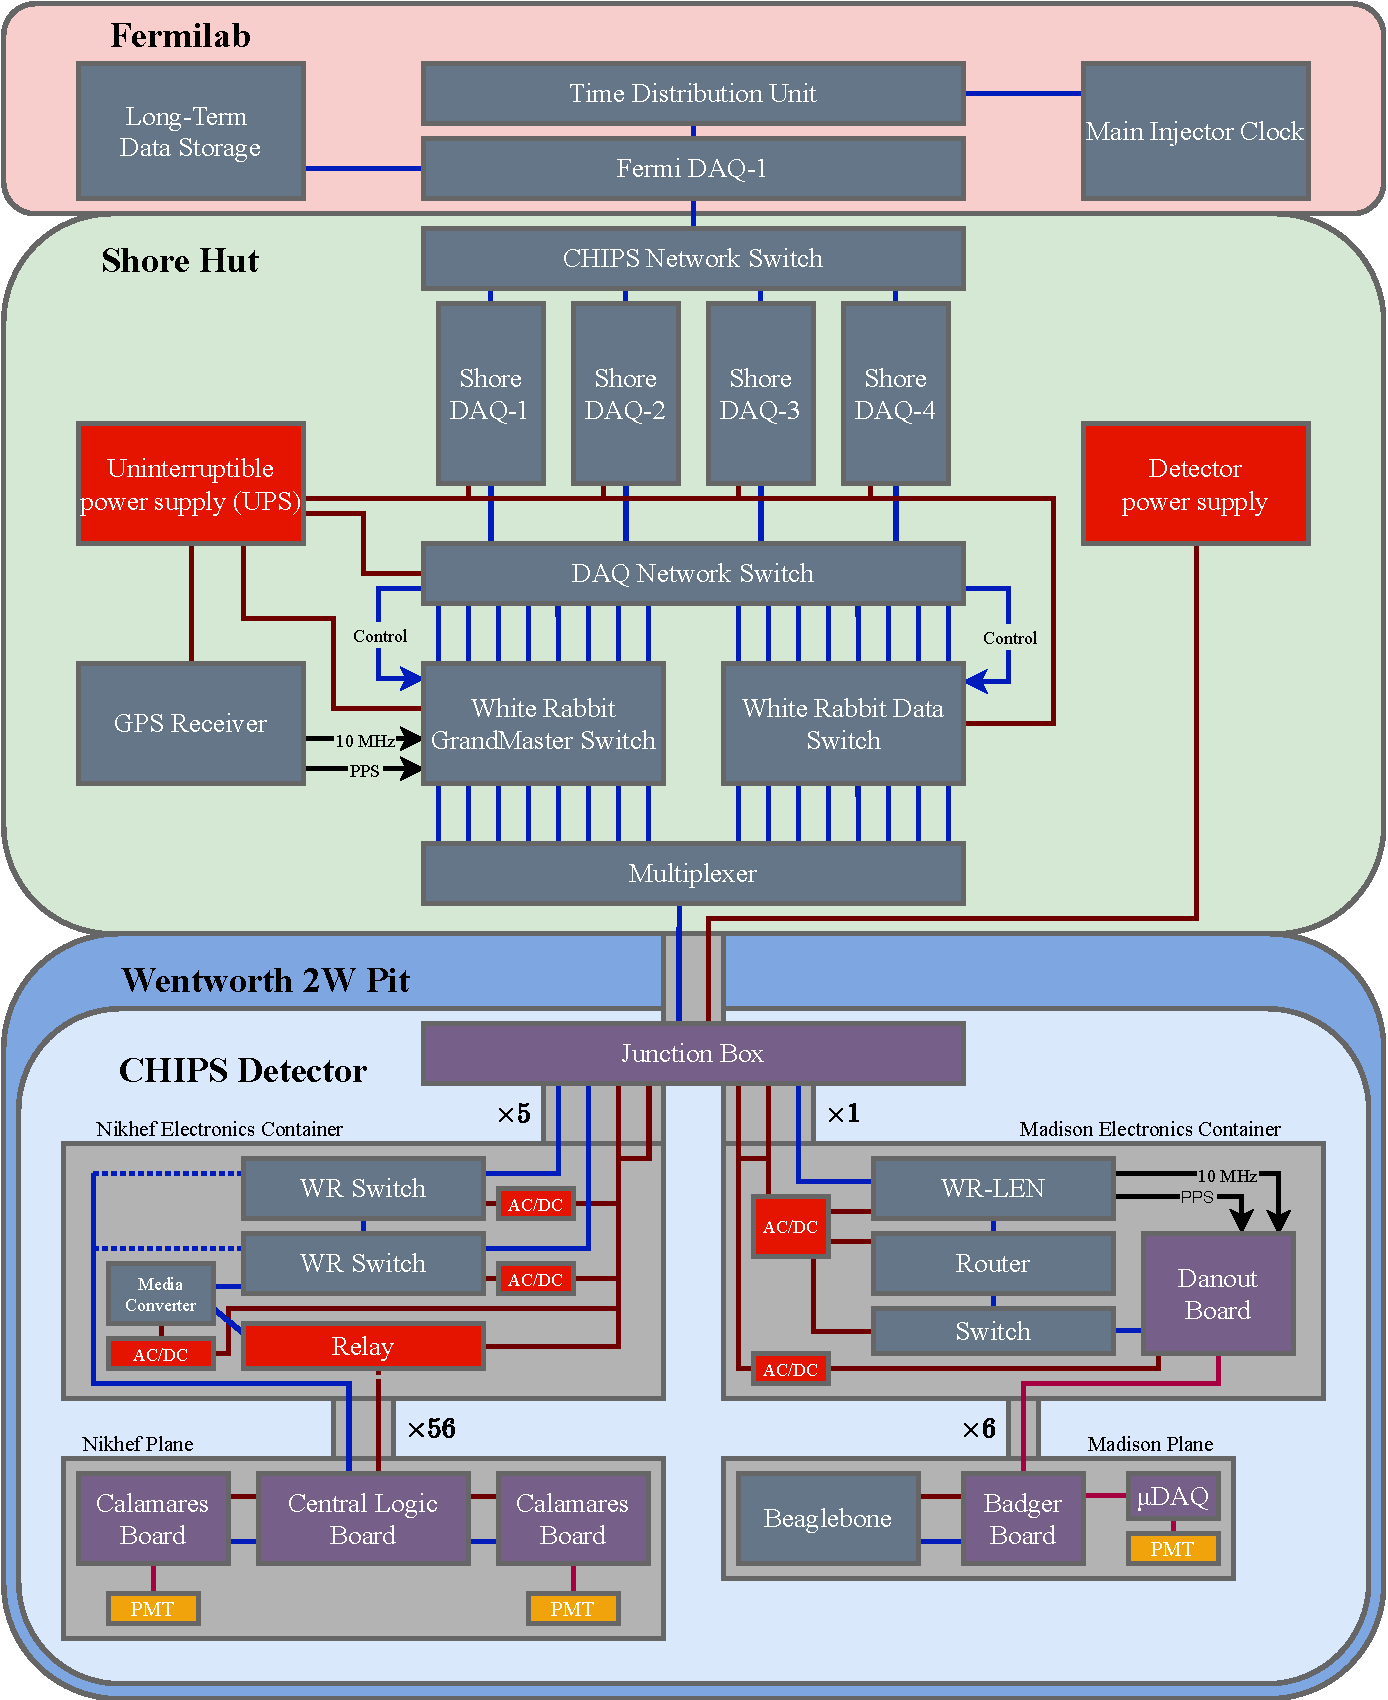
\includegraphics[width=\textwidth]{diagrams/5-daq/daq_detector.pdf}
    \caption[daq detector short]
    {daq detector long}
    \label{fig:daq_detector}
\end{figure}

\subsection{The White Rabbit timing system} %%%%%%%%%%%%%%%%%%%%%%%%%%%%%%%%%%%%%%%%%%%%%%%%%%%%%%
\label{sec:daq_hard_timing} %%%%%%%%%%%%%%%%%%%%%%%%%%%%%%%%%%%%%%%%%%%%%%%%%%%%%%%%%%%%%%%%%%%%%%

REF: White-rabbit papers

\begin{figure} % WHITE-RABBIT SWITCH DIAGRAM %
    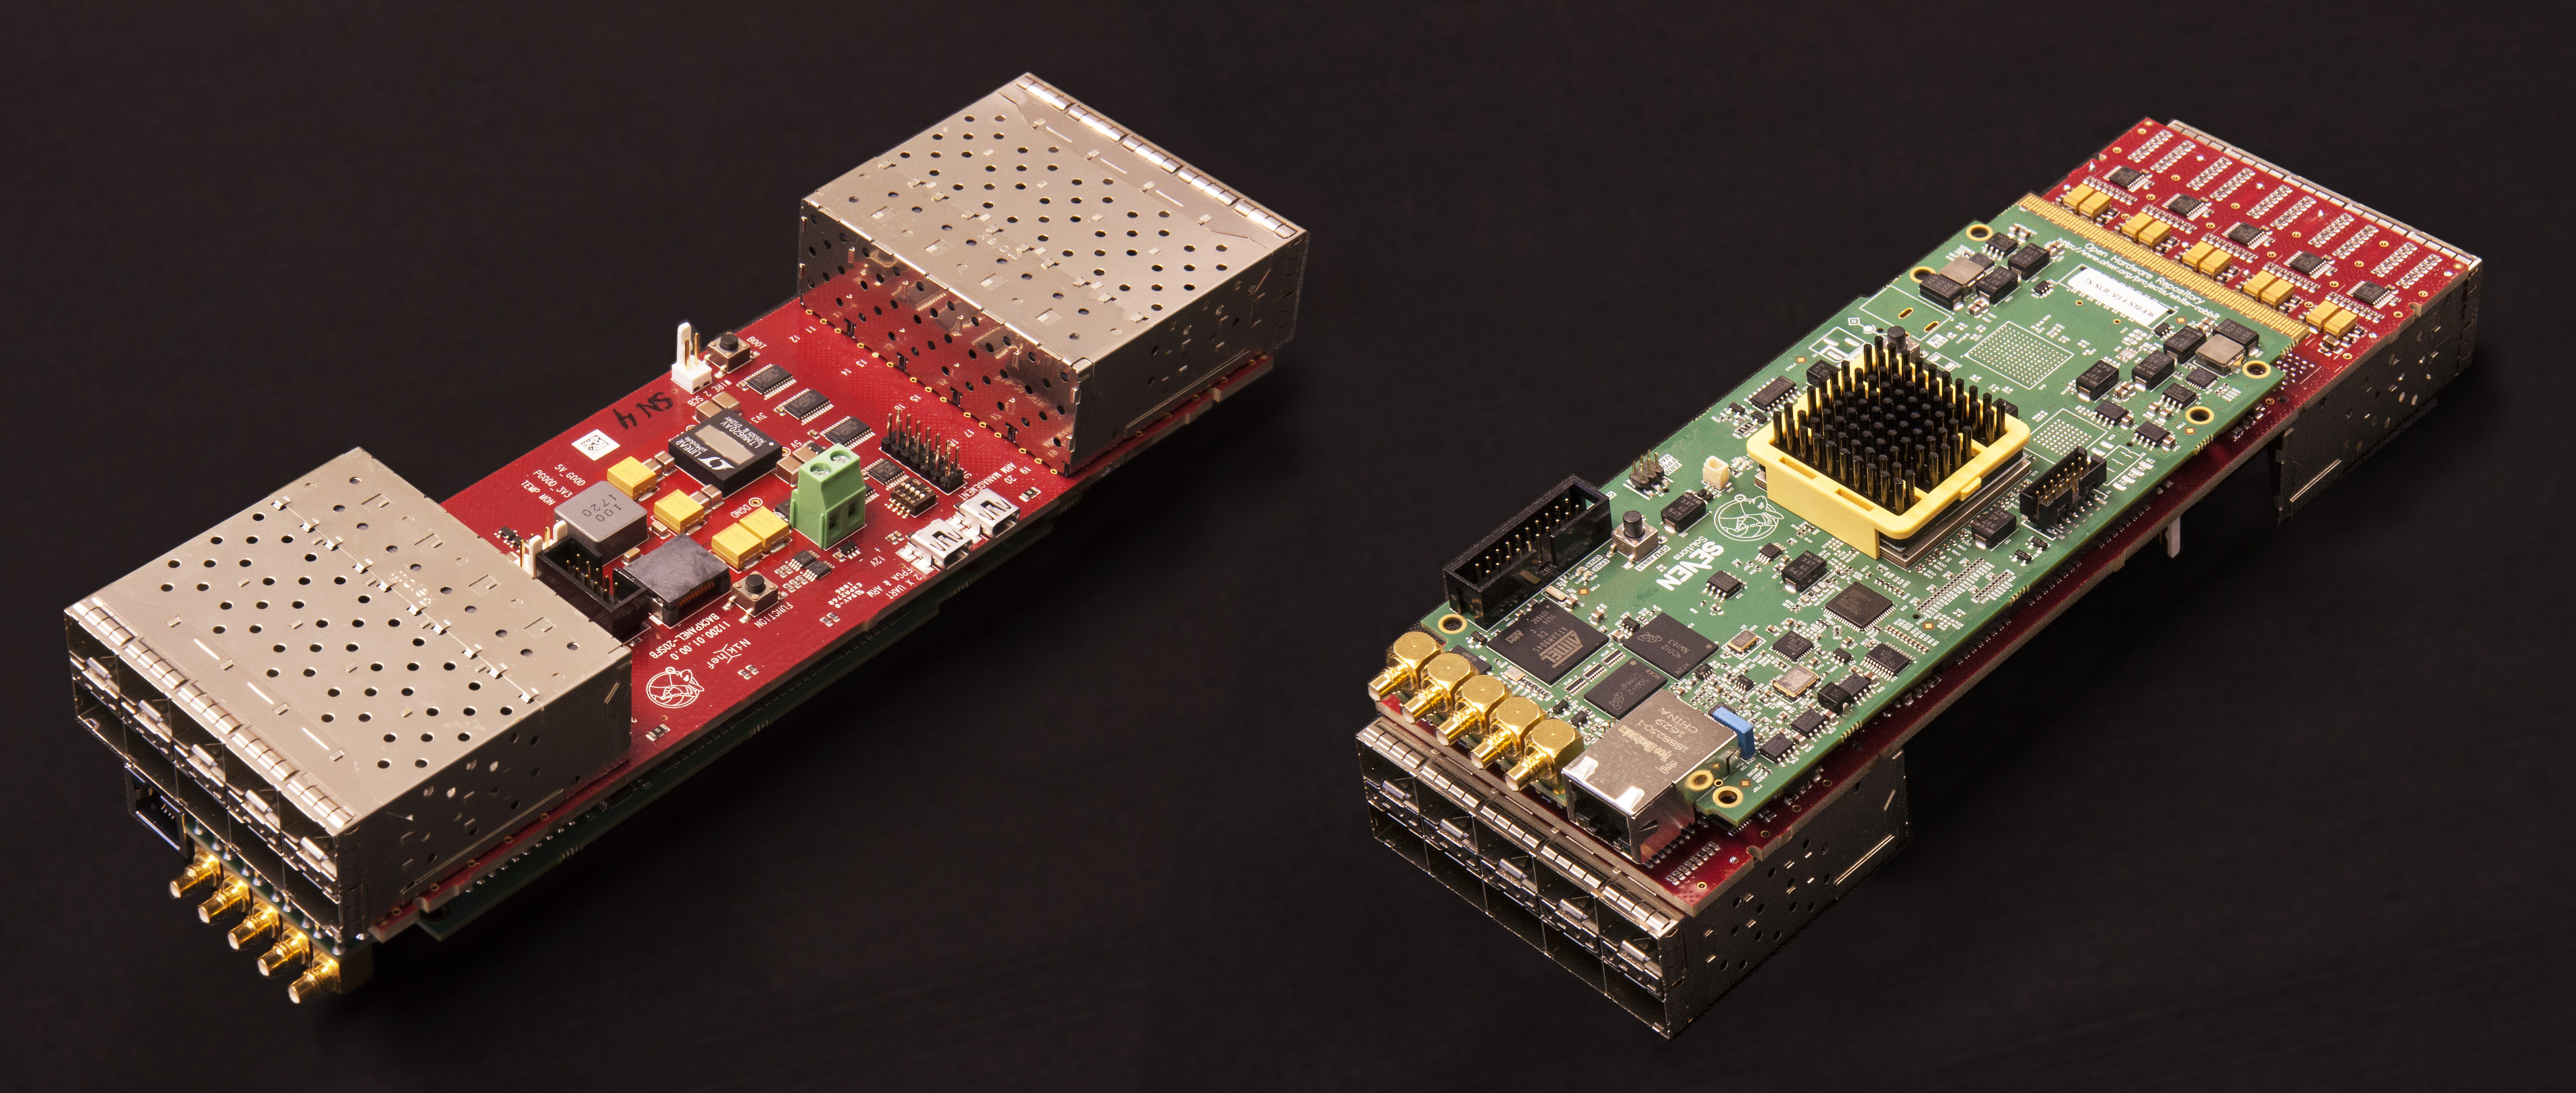
\includegraphics[width=\textwidth]{diagrams/5-daq/wr_switch.jpg}
    \caption[wr switch short]
    {wr switch long}
    \label{fig:wr_switch}
\end{figure}

\begin{figure} % WHITE-RABBIT SYNC DIAGRAM %
    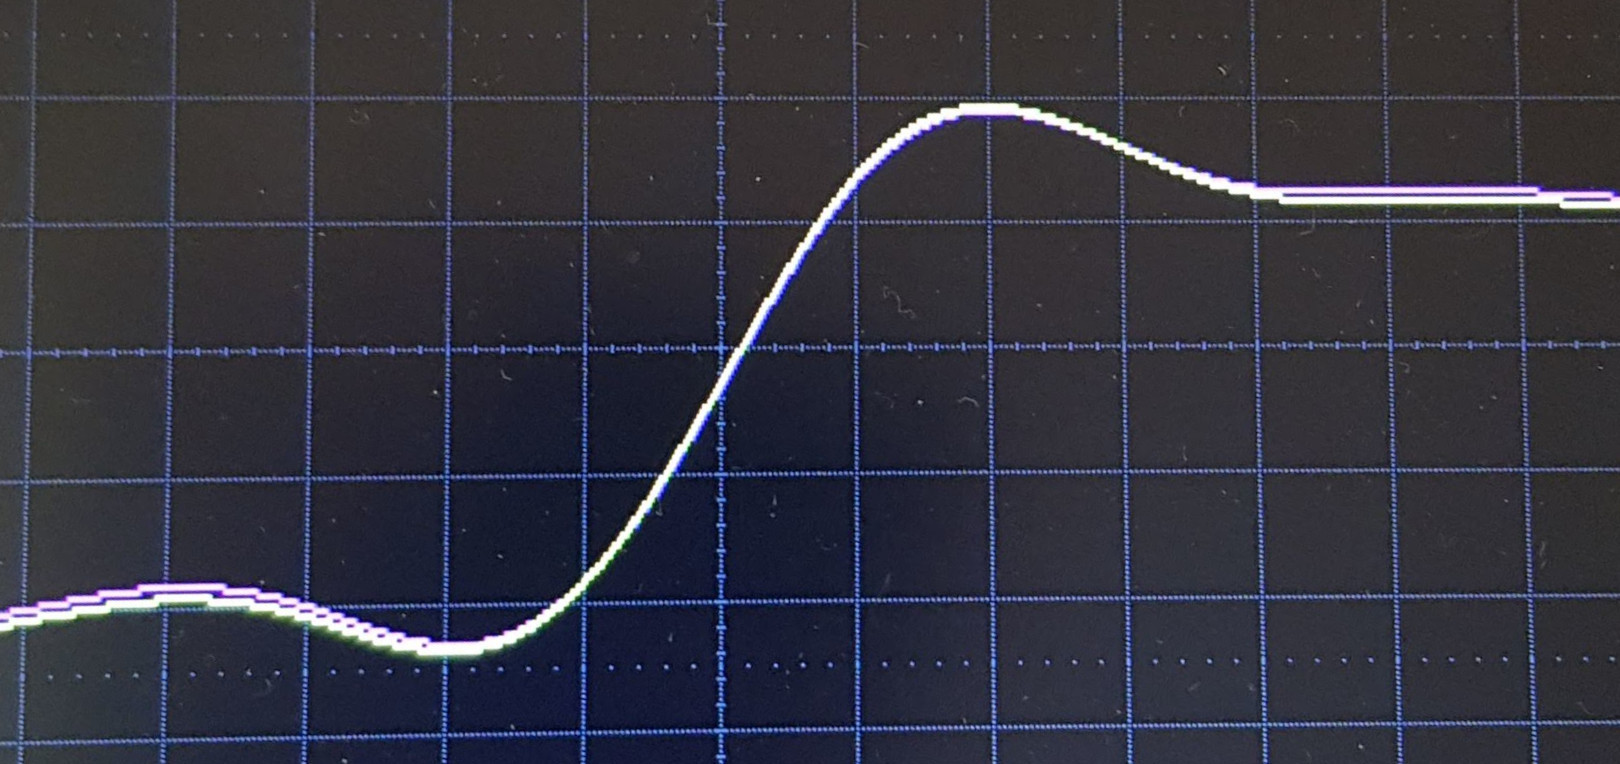
\includegraphics[width=0.8\textwidth]{diagrams/5-daq/sync.jpg}
    \caption[sync short]
    {sync long}
    \label{fig:sync}
\end{figure}

\subsection{Km3NET hardware} %%%%%%%%%%%%%%%%%%%%%%%%%%%%%%%%%%%%%%%%%%%%%%%%%%%%%%%%%%%%%%%%%%%%%
\label{sec:daq_hard_km3net} %%%%%%%%%%%%%%%%%%%%%%%%%%%%%%%%%%%%%%%%%%%%%%%%%%%%%%%%%%%%%%%%%%%%%%

DIAGRAM: Nikhef hardware diagram
REF: PMT time resolution papers
REF: km3net DAQ papers

\begin{figure} % NIKHEF PMT AND CLB DIAGRAM %
    \centering
    \subcaptionbox{nikhef pmt\label{fig:nikhef_pmt}}{%
        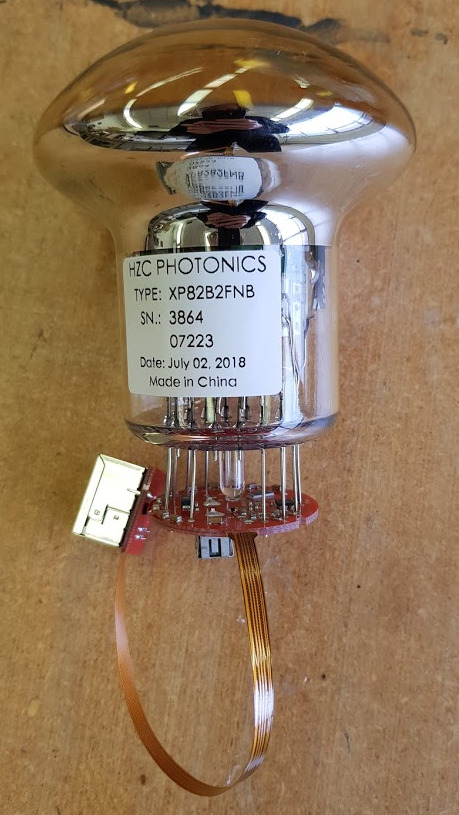
\includegraphics[height=8cm]{diagrams/5-daq/nikhef_pmt.jpg}%
    }
    \quad
    \subcaptionbox{clb\label{fig:clb}}{%
        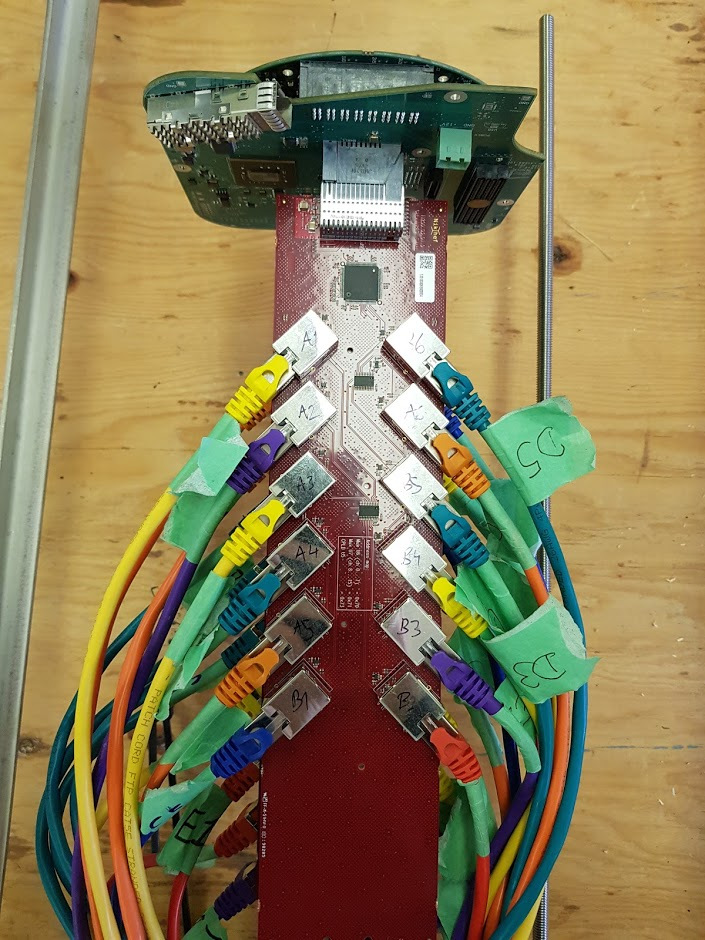
\includegraphics[height=8cm]{diagrams/5-daq/clb.jpg}%
    }
    \caption[The caption]
    {The caption}
\end{figure}

\begin{figure} % CLB ROCKETS DIAGRAM %
    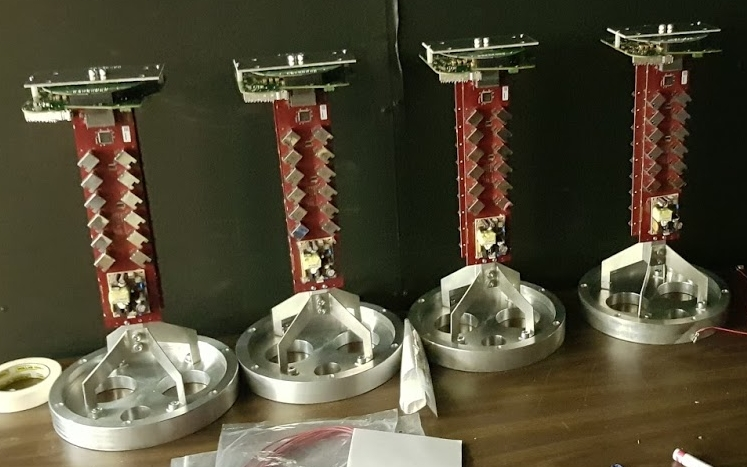
\includegraphics[width=0.6\textwidth]{diagrams/5-daq/rockets.jpg}
    \caption[rockets short]
    {rockets long}
    \label{fig:rockets}
\end{figure}

\subsection{Madison hardware} %%%%%%%%%%%%%%%%%%%%%%%%%%%%%%%%%%%%%%%%%%%%%%%%%%%%%%%%%%%%%%%%%%%%
\label{sec:daq_hard_madison} %%%%%%%%%%%%%%%%%%%%%%%%%%%%%%%%%%%%%%%%%%%%%%%%%%%%%%%%%%%%%%%%%%%%%

DIAGRAM: Madison hardware diagram

\begin{figure} % WR-LEN DIAGRAM %
    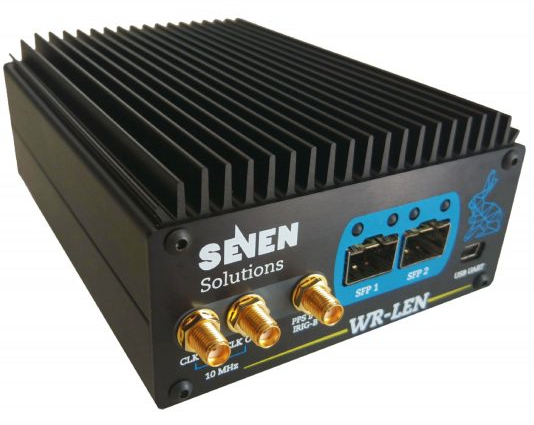
\includegraphics[width=0.8\textwidth]{diagrams/5-daq/wr_len.jpg}
    \caption[wr len short]
    {wr len long}
    \label{fig:wr_len}
\end{figure}

\begin{figure} % TOT DIAGRAM DIAGRAM %
    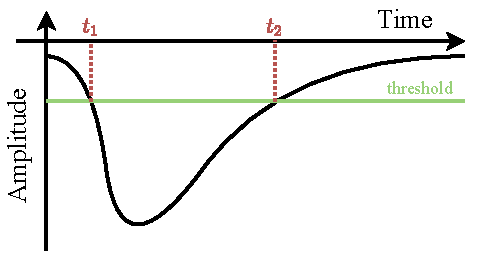
\includegraphics[width=0.6\textwidth]{diagrams/5-daq/tot.pdf}
    \caption[tot short]
    {tot long}
    \label{fig:tot}
\end{figure}

\begin{figure} % BEAGLEBONE AND DANOUT DIAGRAM %
    \centering
    \subcaptionbox{beaglebone\label{fig:beaglebone}}{%
        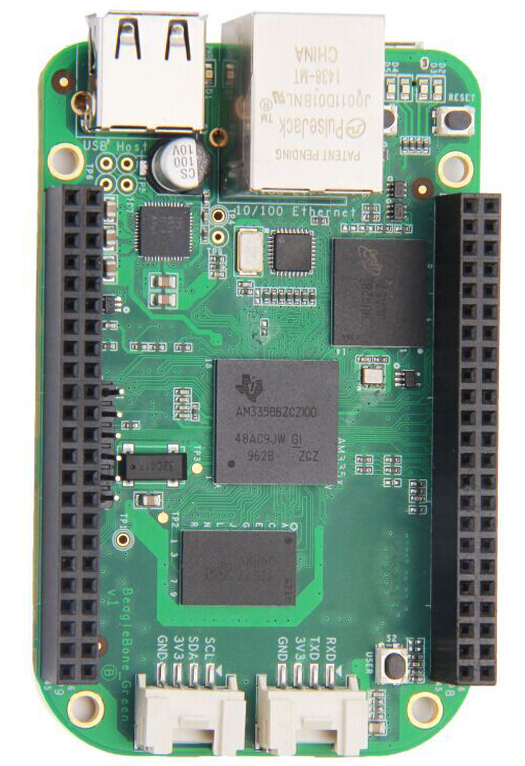
\includegraphics[height=6cm]{diagrams/5-daq/beaglebone.jpg}%
    }
    \quad
    \subcaptionbox{danout\label{fig:danout}}{%
        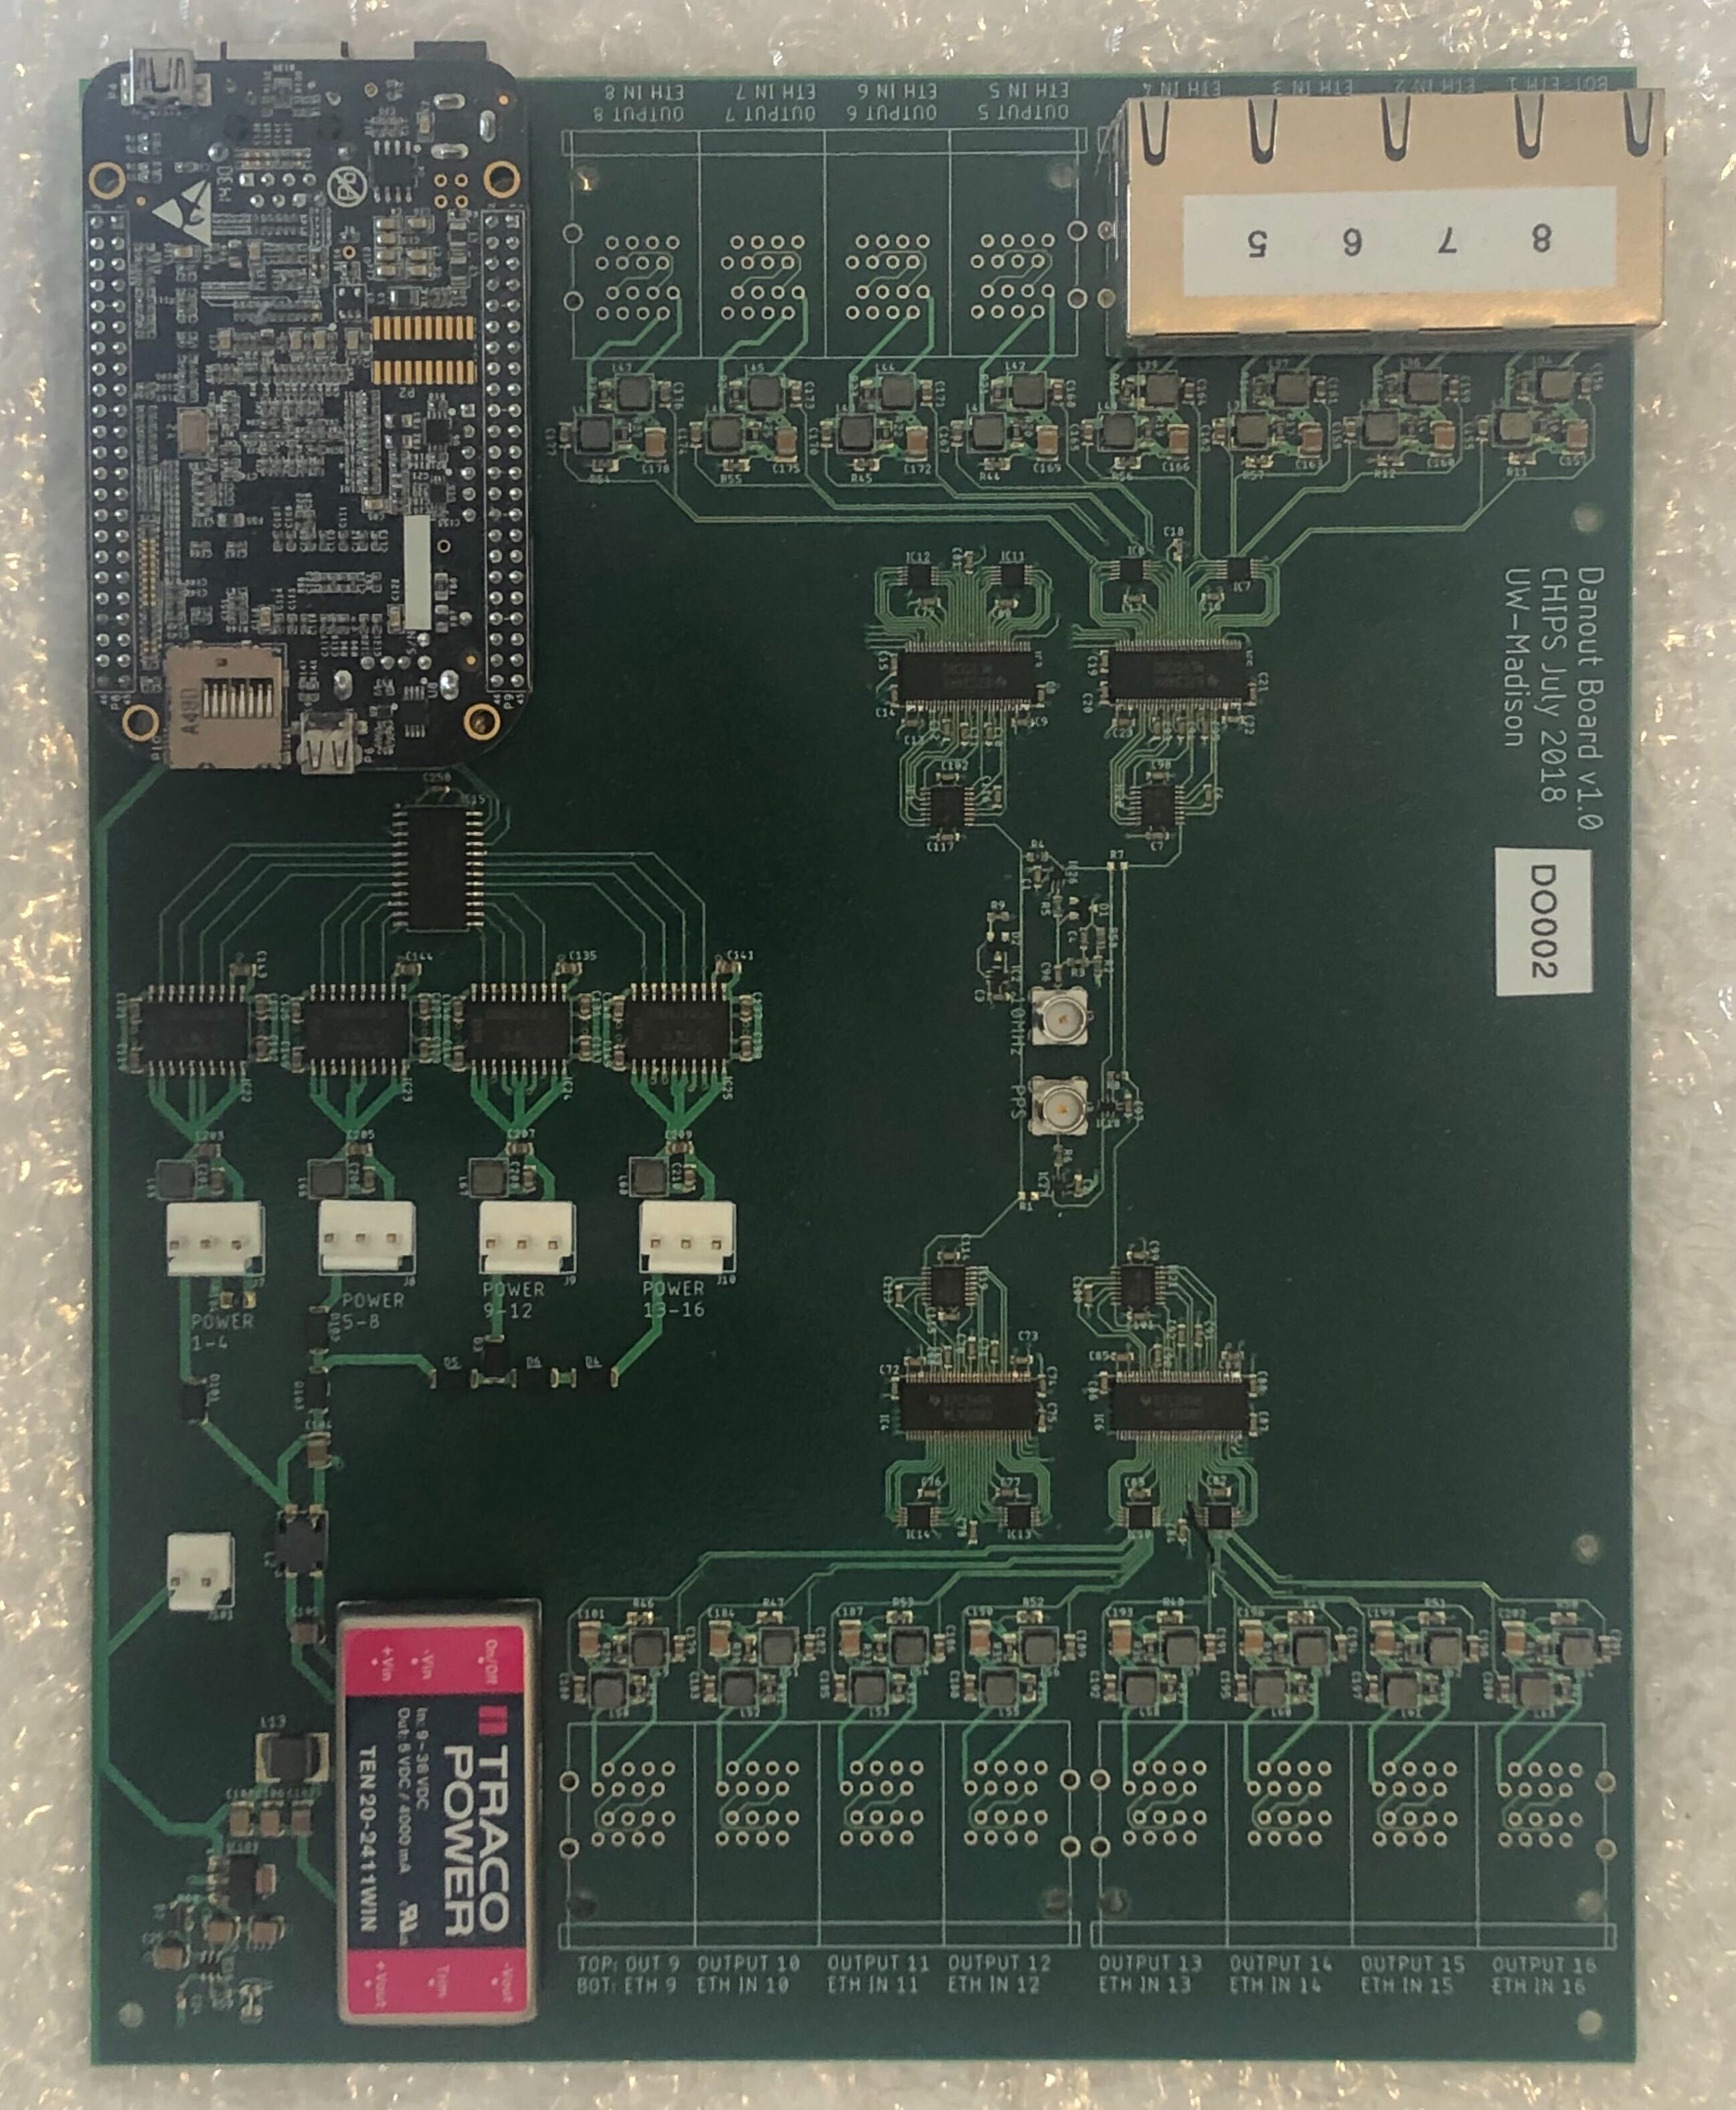
\includegraphics[angle=90, height=6cm]{diagrams/5-daq/danout.jpg}%
    }
    \caption[The caption]
    {The caption}
\end{figure}

\begin{figure} % BADGER BOARD DIAGRAM %
    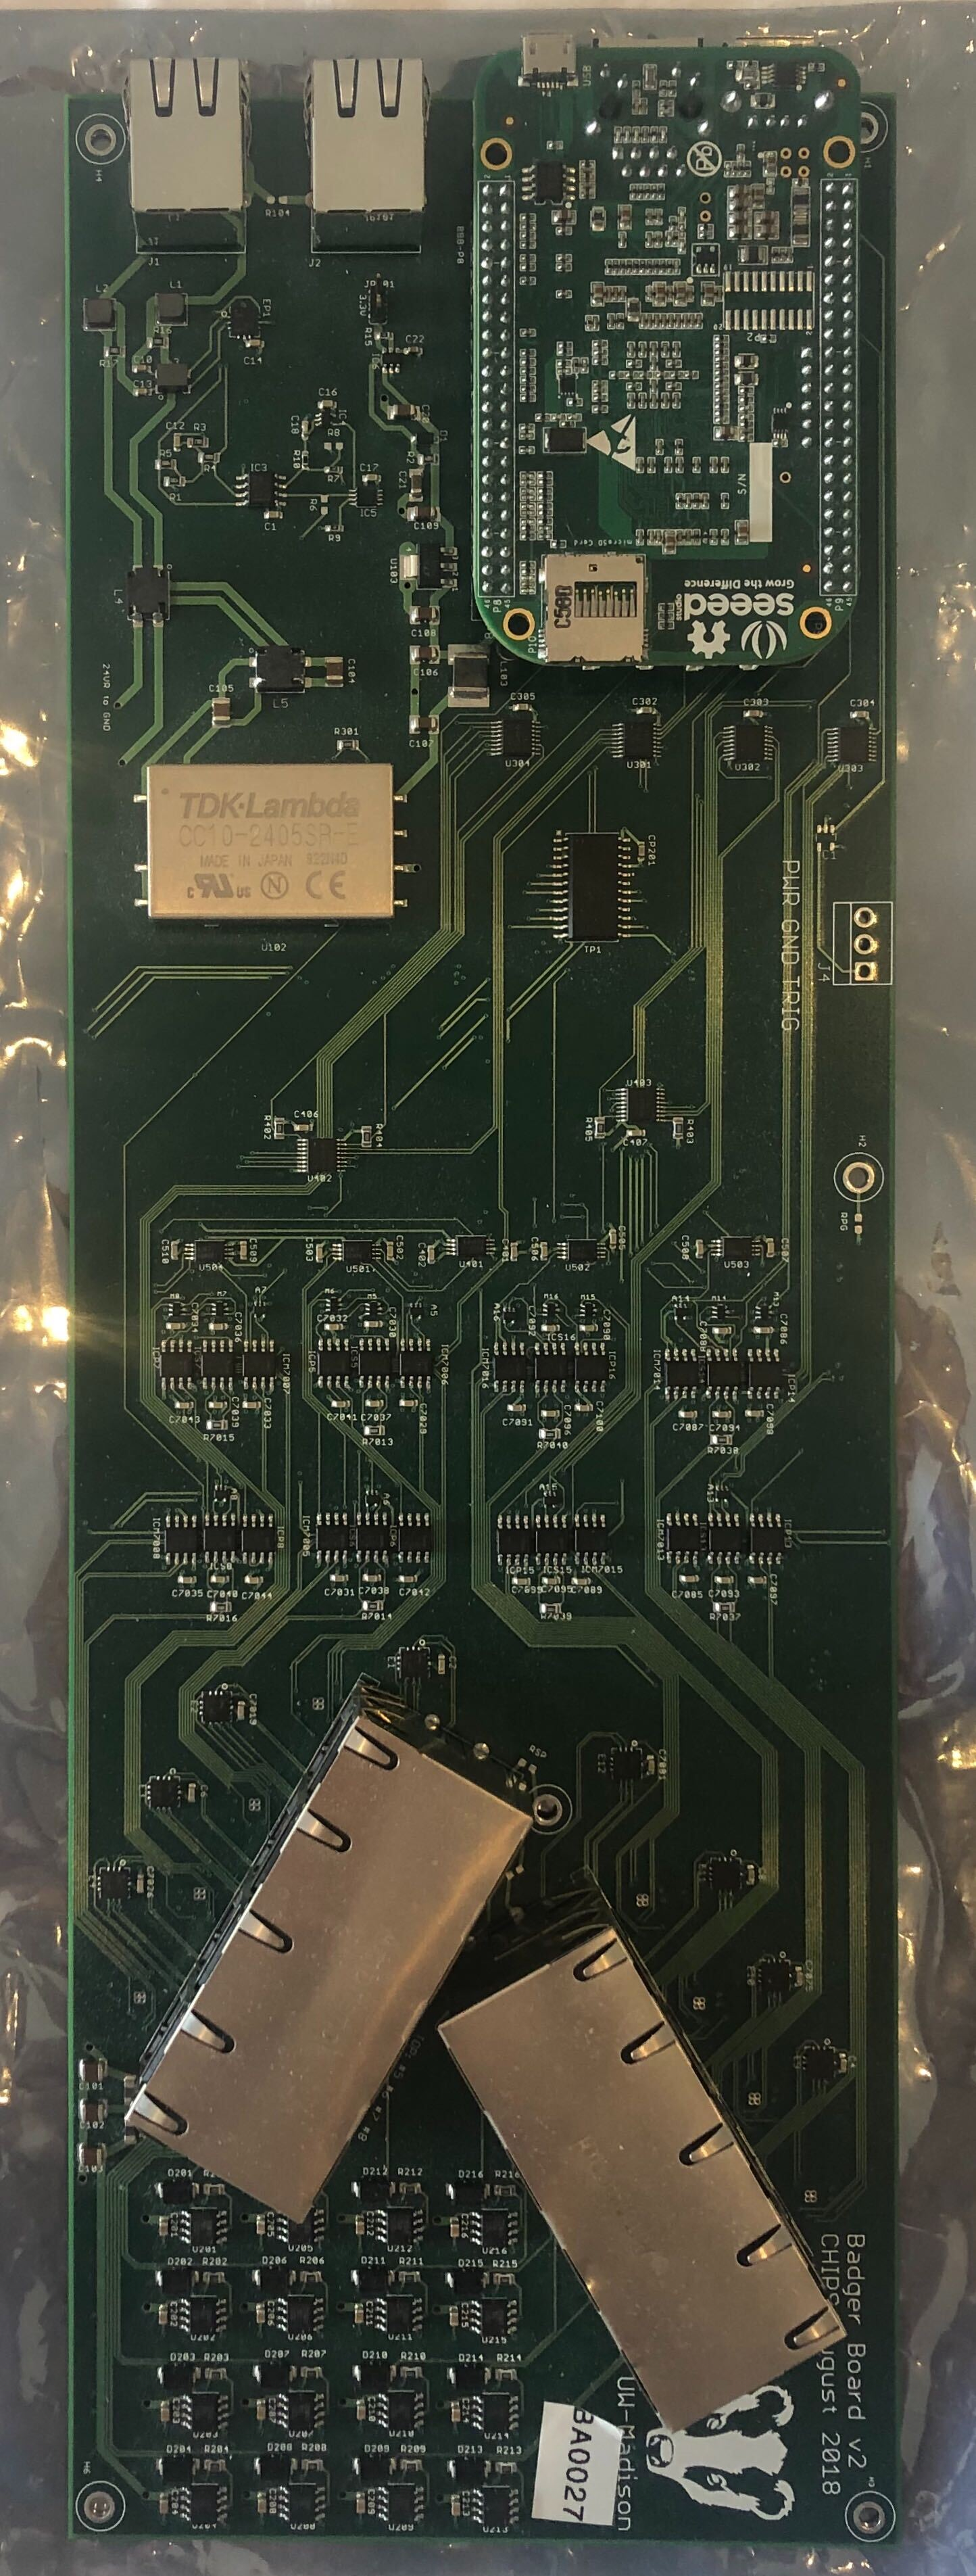
\includegraphics[angle=90,origin=c,width=0.8\textwidth]{diagrams/5-daq/badger.jpg}
    \caption[badger short]
    {badger long}
    \label{fig:badger}
\end{figure}

\subsection{Combined systems} %%%%%%%%%%%%%%%%%%%%%%%%%%%%%%%%%%%%%%%%%%%%%%%%%%%%%%%%%%%%%%%%%%%%
\label{sec:daq_hard_combined} %%%%%%%%%%%%%%%%%%%%%%%%%%%%%%%%%%%%%%%%%%%%%%%%%%%%%%%%%%%%%%%%%%%%

DIAGRAM: Hut Diagram + Jelly box diagram + EC diagrams
DIAGRAM: Manifold layout, box layout in detector

\begin{figure} % WHITE-RABBIT GM SETUP DIAGRAM %
    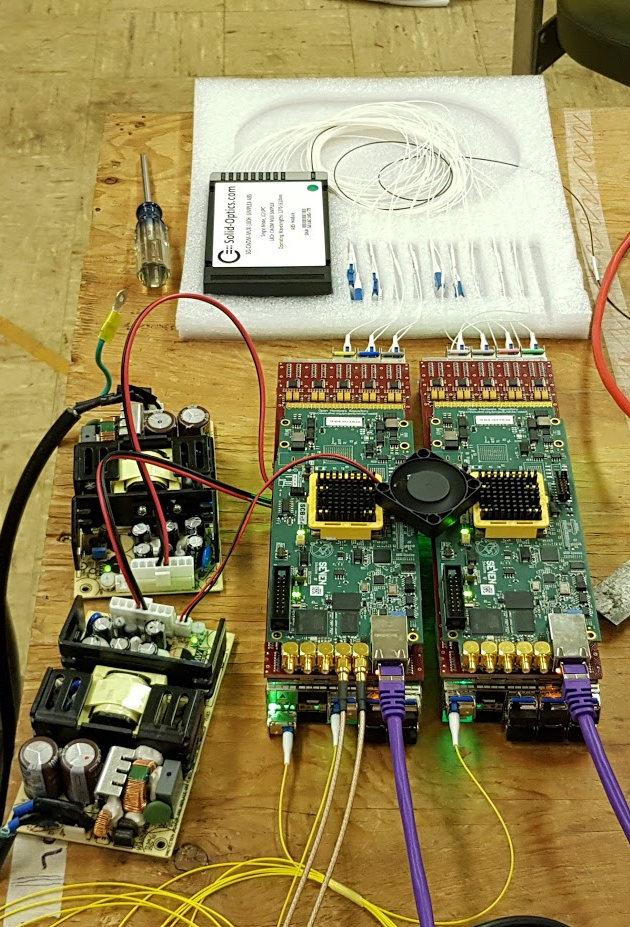
\includegraphics[width=0.8\textwidth]{diagrams/5-daq/wr_gm.jpg}
    \caption[wr gm short]
    {wr gm long}
    \label{fig:wr_gm}
\end{figure}

\section{Software} %%%%%%%%%%%%%%%%%%%%%%%%%%%%%%%%%%%%%%%%%%%%%%%%%%%%%%%%%%%%%%%%%%%%%%%%%%%%%%%
\label{sec:daq_soft} %%%%%%%%%%%%%%%%%%%%%%%%%%%%%%%%%%%%%%%%%%%%%%%%%%%%%%%%%%%%%%%%%%%%%%%%%%%%%

DIAGRAM: Software diagram
DIAGRAM: Finite state machine diagram

\subsection{The beam spill} %%%%%%%%%%%%%%%%%%%%%%%%%%%%%%%%%%%%%%%%%%%%%%%%%%%%%%%%%%%%%%%%%%%%%%
\label{sec:daq_soft_spill} %%%%%%%%%%%%%%%%%%%%%%%%%%%%%%%%%%%%%%%%%%%%%%%%%%%%%%%%%%%%%%%%%%%%%%%

DIAGRAM: Spill server/Fermilab diagram

\subsection{Hit acquisition and handling} %%%%%%%%%%%%%%%%%%%%%%%%%%%%%%%%%%%%%%%%%%%%%%%%%%%%%%%%
\label{sec:daq_soft_hits} %%%%%%%%%%%%%%%%%%%%%%%%%%%%%%%%%%%%%%%%%%%%%%%%%%%%%%%%%%%%%%%%%%%%%%%%

\subsection{Detector and data quality monitoring} %%%%%%%%%%%%%%%%%%%%%%%%%%%%%%%%%%%%%%%%%%%%%%%%
\label{sec:daq_soft_monitor} %%%%%%%%%%%%%%%%%%%%%%%%%%%%%%%%%%%%%%%%%%%%%%%%%%%%%%%%%%%%%%%%%%%%%

REF: Elasticsearch paper

\begin{figure} % MONITORING DIAGRAM %
    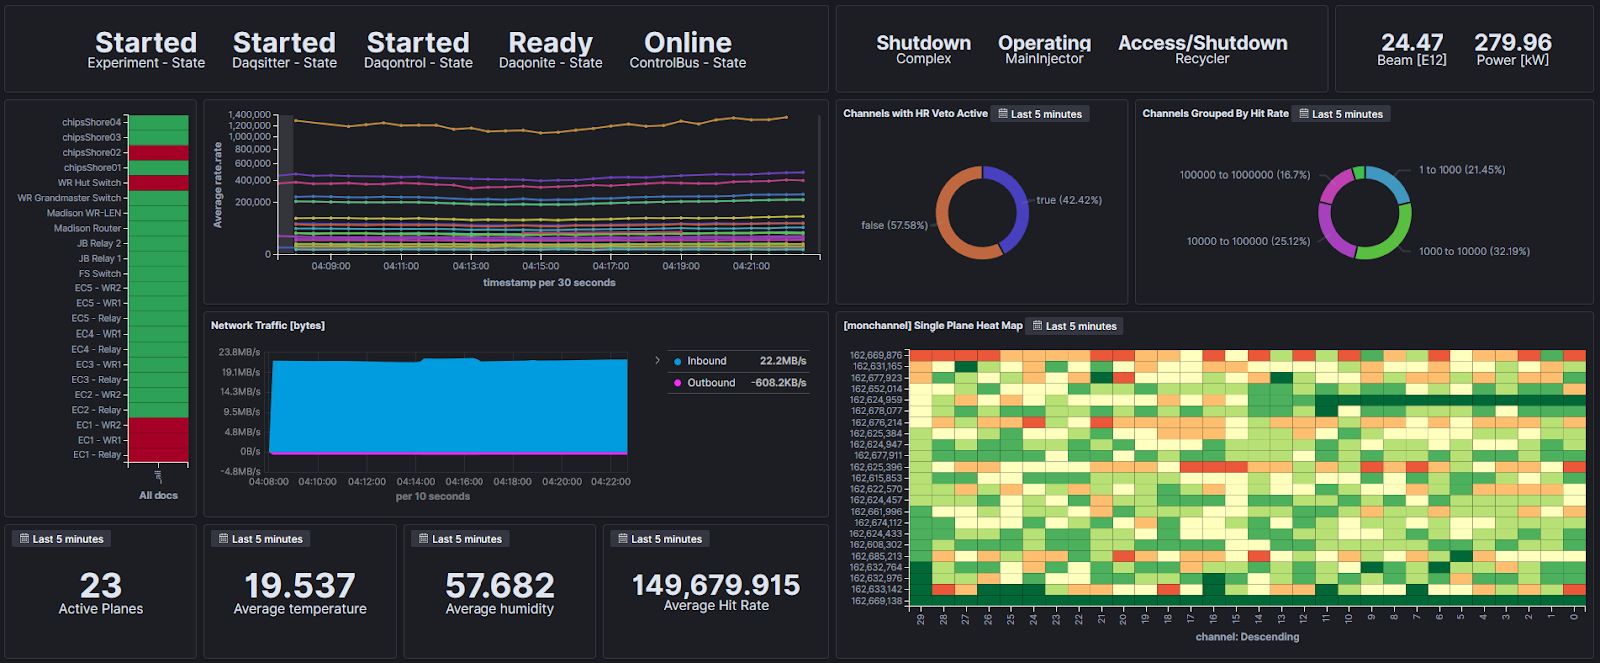
\includegraphics[width=\textwidth]{diagrams/5-daq/monitoring.png}
    \caption[monitoring short]
    {monitoring long}
    \label{fig:monitoring}
\end{figure}